\chapter*{Introduction}
\addcontentsline{toc}{chapter}{Introduction}

\section*{Software Quality Importance}
\addcontentsline{toc}{section}{Software Quality Importance}

A high quality in pieces of software should be the objective for programmers of any competence level to aim for, it shows that the software is less likely to contain performance issues or even to fail when compared to a poor quality one. This leads end-users to have a more positive experience, which leads them to keep using the software software and to consider the developers s \textit{reliable}. 

\section*{AI Growing Role in Software Development}

\addcontentsline{toc}{section}{AI Growing Role in Software Development}

AI has made it's way in many different aspects of our lives, from the most mundane of activities to the most exciting ones, and coding is also part of this AI bubble. 

Today, most softwares are partially, or even in their entirety, coded with the assistance of AI tools. More often than not, this may introduce risks in reliability, as opposed to when the program is written by a human being.

\begin{multicols}{2}
\begin{figure}[H]
    \centering
    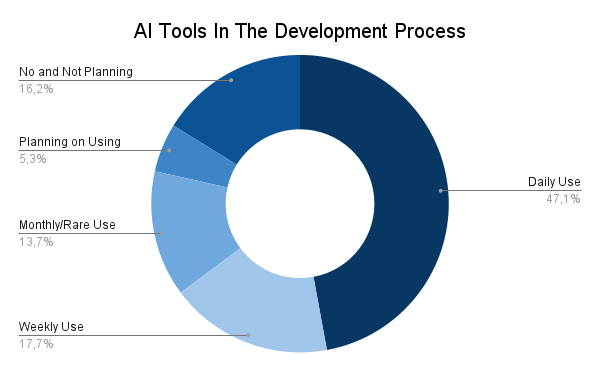
\includegraphics[width=0.88\linewidth]{images/AI Tools In The Development Process.png}
    \caption{Percentage of Users Using AI (Source: Stack Overflow Developer Survey 2025 \cite{stackoverflow2025}).}
    \label{fig:PeopleAI_Graph}
\end{figure}

As we can see in Figure \ref{fig:PeopleAI_Graph} more than 45\% of people that took part in this survey use AI on a daily basis. 
Let's also notice that \textit{more} than 80\% of developers have already integrated or are planning on integrating AI in their programming life.
\end{multicols}



\section*{Survey's Goals}
\addcontentsline{toc}{section}{Survey's Goals}

The goal of this survey to analyze the role that AI tools have in supporting software quality during the process of development. Specifically, it focuses on AI-based systems used for code generation, analysis, and for test automation, without considering chatbots such as ChatGPT or Deepseek.

The objective is to give an overview of these tools, discuss solutions, and to analyze the impact they have on software quality characteristics like maintainability, correctness, and security. As well as, to highlight both the benefits and the limitations of AI-assisted development tools.

\section*{Structure}
\addcontentsline{toc}{section}{Structure}

The survey from this point forward is structured like so. Chapter 1 introduces the background and fundamental concepts related to AI and software quality. Chapter 2 provides a short classification of AI tools used in programming. Chapters 3 through 5 go through code generating AIs, code analysis AI, and test automation AIs respectively. Finally chapter 6 discusses the future directions and open challenges that enabling AI in software quality holds.